%% Scientific Reports submission — single column, numbered citations
\documentclass[12pt,a4paper]{article}

\usepackage{amsmath,amssymb,amsfonts}
\usepackage{graphicx}
\usepackage{booktabs}
\usepackage{multirow}
\usepackage{microtype}
\usepackage[T1]{fontenc}
\usepackage[utf8]{inputenc}
\usepackage[margin=2.5cm]{geometry}
\usepackage{setspace}
\usepackage{caption}
\usepackage{subcaption}
\usepackage[numbers,sort&compress]{natbib}
\usepackage[colorlinks=true,linkcolor=blue,citecolor=blue,urlcolor=blue]{hyperref}
\usepackage{xcolor}
\usepackage{lineno}
\linenumbers

\setstretch{1.5}

\begin{document}

% ─────────────────────────────────────────────────────────────────────────────
\title{\textbf{Predicting Speech-in-Noise Performance Beyond the Pure-Tone
Audiogram: A Machine Learning Benchmark on the Oldenburg Hearing Health
Record}}

\author{Ryan Yi Sheng Neo\\[0.4em]
\small Independent Researcher\\[0.2em]
\small \href{mailto:realryanneo@gmail.com}{realryanneo@gmail.com}}
\date{}
\maketitle

% ─────────────────────────────────────────────────────────────────────────────
\begin{abstract}
Pure-tone audiometry is the standard characterisation of hearing loss, yet
audiogram thresholds explain only part of real-world speech understanding.
To our knowledge, we present the first systematic machine learning (ML)
benchmark on the Oldenburg Hearing Health Record (OHHR), a publicly available
dataset of 581 adults with pure-tone audiograms, adaptive loudness scaling,
speech-in-noise tests, cognitive assessments, and self-report measures.
Five feature blocks (1--41 features) were evaluated using Ridge regression,
Random Forest, LightGBM, and a multilayer perceptron under 10-fold
cross-validation.  For predicting Digit Triplet Test speech-reception
threshold, a binaural four-frequency pure-tone average achieves $R^2=0.71$;
the full battery with Random Forest reaches $R^2=0.81$
(MAE\,=\,1.23\,dB~SNR).  SHAP analysis identifies better-ear PTA, age, and
loudness-growth slope as the most informative features.  The benefit of
richer feature sets is largest in mild hearing loss (26--40\,dB), where the
audiogram alone explains only 9\% of speech-in-noise variance and the full
battery achieves 37\%.  Poor speech-in-noise performers are classified with
AUROC\,=\,0.978 (Brier\,=\,0.053).  Cross-cohort validation on NHANES
2017--18 ($N=859$) shows that age adds discriminative power for
self-reported hearing difficulty (AUROC: 0.758 $\to$ 0.815).  All code is
released openly.
\end{abstract}

\textbf{Keywords:} hearing loss, speech in noise, machine learning,
audiology, OHHR, SHAP, calibration, audiogram, loudness scaling

\vspace{1em}
\hrule
\vspace{1em}

% ─────────────────────────────────────────────────────────────────────────────
\section{Introduction}

Hearing loss is the third most prevalent chronic condition globally, affecting
an estimated 1.6 billion people, with projections reaching 2.5 billion by
2050\cite{who2021}.  Its primary clinical characterisation---the pure-tone
audiogram---measures the softest audible tones across standard frequencies,
yet the audiogram is an incomplete account of real-world hearing function.
A substantial fraction of adults with normal or near-normal audiometric
thresholds report significant difficulty understanding speech in noise
(SIN)\cite{Plack2014HiddenHL}, a phenomenon linked to cochlear synaptopathy
and suprathreshold auditory processing deficits.  Conversely, individuals
with similar audiograms can differ markedly in everyday communicative success
owing to differences in cognitive capacity, loudness recruitment, or perceived
hearing quality\cite{Gatehouse2004SSQ}.

Predicting SIN performance from audiological measurements has therefore
attracted sustained research interest.  Classical regression studies
established that pure-tone average (PTA) at 0.5--4\,kHz explains roughly
50--70\% of SIN variance in adult cohorts\cite{Smoorenburg1992}, and
subsequent work has sought to identify which additional measurements close
the remaining gap.  Cognitive factors---particularly working memory
capacity---have repeatedly been shown to contribute independently of
audiometric thresholds, especially for linguistically demanding sentence
tasks\cite{Ng2015CognitionSIN,Lunner2003WM}.  Suprathreshold measures of
loudness growth derived from adaptive categorical loudness scaling (ACALOS)
capture outer hair cell integrity beyond what threshold audiometry
detects\cite{Brand2002}, and several groups have found that loudness
parameters add predictive value for SIN over and above PTA alone.

Recent machine learning (ML) work on large clinical databases has largely
confirmed the PTA--SIN relationship while achieving modest performance
improvements through non-linear modelling\cite{Gathman2023}.
However, most published ML approaches have used narrow feature sets
(PTA-only or demographics plus PTA), have not reported calibrated
probabilistic predictions, have rarely examined severity-stratified
utility, and have been applied to proprietary datasets that preclude
direct benchmarking.  The clinical question of whether extended audiological
assessments---beyond the audiogram---justify their administrative burden
for functional hearing counselling therefore remains open.

The recently published Oldenburg Hearing Health Record
(OHHR)\cite{OHHR2025} offers a unique opportunity to address these gaps.
OHHR is an open, CC~BY~4.0 dataset of 581 adults (aged 18--86) containing
air-conduction audiograms, adaptive categorical loudness scaling, digit-triplet
and G\"{o}ttingen sentence speech-in-noise tests, cognitive assessments
(DemTect, WortSchatz), socio-economic indicators, and self-report
questionnaires.  Its multimodal design makes it ideal for disentangling
audiometric, auditory-processing, cognitive, and demographic contributions
to functional hearing in a reproducible benchmark setting.

Our contributions are: (i) the first systematic ML benchmark on OHHR,
comparing five feature blocks spanning 1--41 features and four model
families; (ii) a SHAP-based decomposition of the most informative features
beyond the pure-tone audiogram; (iii) severity-stratified analysis showing
that the clinical benefit of extended assessment is concentrated in mild
hearing loss; (iv) calibrated probabilistic risk predictions for clinical
screening; (v) a neural MLP baseline confirming that tree-ensemble
performance is not capacity-limited on this dataset; and (vi) partial cross-cohort construct validation on NHANES, showing that
OHHR-trained models transfer to self-reported hearing difficulty in an
independent general-population sample and corroborating the importance of
age beyond the audiogram.
All code, feature engineering scripts, and pre-trained model weights are
released openly to support reproducible computational audiology research.

% ─────────────────────────────────────────────────────────────────────────────
\section{Materials and Methods}

\subsection{Dataset}

The Oldenburg Hearing Health Record (OHHR, version 2.0, Zenodo record
16919812\cite{OHHR2025}) contains data from 581 adults (255~female,
326~male; age $M=67.5\pm12.0$\,years, range 19--86) collected between 2013
and 2015 at the H\"{o}rzentrum Oldenburg, Germany.  The cohort spans the
full range of clinically relevant hearing loss (better-ear PTA4:
$M=31.3\pm17.2$\,dB~HL), with 39\% having near-normal thresholds
($\leq$25\,dB) and 31\% having moderate-to-severe loss ($>$40\,dB).
Participant characteristics are summarised in Supplementary Table~S1.
All participants gave written informed consent; data are anonymised and
released under CC~BY~4.0; this study requires no additional ethics approval
as it analyses a pre-existing publicly available dataset.

\subsection{Feature Extraction}

We constructed 41 features organised into five progressively richer
\textit{feature blocks}:

\textbf{Block~A} (1~feature): binaural four-frequency pure-tone average
(PTA4 mean: mean of left- and right-ear PTA4, where PTA4\,=\,mean of 0.5,
1, 2, and 4\,kHz air-conduction thresholds).

\textbf{Block~B} (14~features): full air-conduction hearing threshold level
(HTL) audiogram, comprising thresholds at seven frequencies (250--4000\,Hz)
for each ear.

\textbf{Block~C} (23~features): Block~B plus nine loudness-scaling parameters
derived from the ACALOS procedure---the Brand \& Hohmann (2002)
loudness growth function parameters $m_\text{low}$, $m_\text{high}$, and
$m_\text{cut}$ per ear\cite{Brand2002}, plus mean UCL per ear and inter-ear
MCL asymmetry.

\textbf{Block~D} (25~features): Block~C plus DemTect total score (cognitive
screening, 0--18) and WortSchatz verbal intelligence score.

\textbf{Block~E} (41~features): Block~D plus age, sex, education, net income,
hearing aid supply status, hearing loss history flags, and derived audiogram
summaries (better-ear, worse-ear, binaural-mean, and inter-ear-asymmetry
PTA4; high-frequency slope per ear).

Missing values (maximum 3.8\% per feature) were imputed with the
training-fold median; continuous features were standardised for Ridge
regression and the MLP.

\subsection{Cross-Cohort Validation Data}
\label{sec:nhanes}

For partial external validation we used the NHANES 2017--2018 audiometry
module (AUX\_J), hearing questionnaire (AUQ\_J), and demographics
(DEMO\_J)\cite{NHANES2018}.  NHANES audiometric testing in that cycle was
restricted to adults aged 70--80~years.  After requiring valid pure-tone
thresholds at 0.5, 1, 2, and 4\,kHz bilaterally, the analysis sample
comprised $N=859$ participants.  Shared features were: bilateral PTA4
summaries (better, worse, mean, asymmetry), age, and sex.  The primary
validation outcome was AUQ054 (\textit{``How good is your hearing?''},
6-point scale: 1\,=\,excellent, 2\,=\,good, 3\,=\,a little trouble,
4\,=\,moderate trouble, 5\,=\,a lot of trouble, 6\,=\,deaf), dichotomised as
$\geq$3 (any hearing trouble; positive rate 48.8\%).  A secondary outcome was AUQ101
(\textit{``Difficulty hearing in noise?''}, 5-point scale coded
1\,=\,Always \ldots 5\,=\,Never), dichotomised as $\leq$2 (always or
usually; positive rate 26.7\%).  Both outcomes are self-report proxies; the
analysis constitutes partial construct validation rather than replication of
the OHHR speech-in-noise endpoint.  Classifiers trained on OHHR were applied
without retraining to the NHANES sample.

\subsection{Prediction Targets}

\textbf{Primary (regression)}: Digit Triplet Test (DTT) speech-reception
threshold (SRT, dB~SNR), measured binaurally in free field at 65\,dB~SPL
noise ($M=-4.6$\,dB, $SD=4.2$\,dB).  Lower SRT indicates better performance.

\textbf{Secondary (regression)}: G\"{o}ttingen Sentence Test (GST) SRT
($M=-1.5$, $SD=3.1$\,dB).

\textbf{Classification}: \textit{Poor SIN} defined as DTT
SRT\,$>$\,$-2$\,dB~SNR (21.0\% prevalence, $n=122$).  This threshold lies
approximately 2.6\,dB above the cohort mean ($-4.6$\,dB) and corresponds to
the upper tail of the distribution where speech intelligibility degrades
markedly in typical listening environments; similar DTT-based cut-offs have
been used in prior clinical screening studies for speech-in-noise deficits.

\subsection{Models and Evaluation}

Four model families were evaluated for regression: \textbf{Ridge regression}
($\alpha=1$); \textbf{Random Forest} (RF; 200~trees, $\sqrt{p}$ features,
min.~leaf~5); \textbf{LightGBM} (500~estimators, learning rate~0.05,
31~leaves, $L_2=1.0$); and a \textbf{multilayer perceptron} (MLP;
256/128/64~units, batch normalisation, dropout~0.25, Adam optimiser,
early stopping; patience~30).  For classification, \textbf{logistic
regression} (LR) was additionally evaluated.

Regression performance was quantified as $R^2$ and MAE under 10-fold
cross-validation (CV); per-fold values were retained for statistical testing.
Bootstrap 95\% confidence intervals (2000~resamples, concatenated OOF
predictions) were computed for each model's Block~E $R^2$.  Pairwise model
and block comparisons used the Wilcoxon signed-rank test on the 10~fold-level
$R^2$ values (two-sided; significance threshold $\alpha=0.05$; sample
size~$n=10$ folds is sufficient to detect large effects but limits power
for subtle improvements).  Classification performance was evaluated via
AUROC, AUPRC, and Brier score under 10-fold stratified CV; AUROC confidence
intervals and pairwise tests used the bootstrap ($n=2000$ resamples).

\textbf{Feature importance}: SHAP values\cite{Lundberg2017SHAP} were
computed for the LightGBM model trained on Block~E features.  Stability
across the 10~CV folds was quantified by the coefficient of variation (CV)
of the per-fold mean absolute SHAP value.

\textbf{Severity subgroup analysis}: Participants were stratified by
better-ear PTA4 into four severity groups ($\leq$25, 26--40, 41--60,
$>$60\,dB~HL) and within-stratum 5-fold Ridge CV $R^2$ was computed for
Block~A and Block~E.

\textbf{Minimal predictor analysis}: Starting from the SHAP feature ranking,
features were added one at a time in importance order and 10-fold
LightGBM CV $R^2$ was tracked, identifying the smallest set achieving
near-maximal performance.

% ─────────────────────────────────────────────────────────────────────────────
\section{Results}

\subsection{DTT SRT Regression Benchmark}

Table~\ref{tab:benchmark} and Fig.~\ref{fig:benchmark} summarise regression
performance.  The binaural PTA4-mean baseline (Block~A) already explains
70.8--71.9\% of DTT SRT variance across all models---a remarkably efficient
single-feature baseline.  Extending to the full audiogram (Block~B) yields
a clear gain for ensemble methods (RF: $R^2=0.790$, LightGBM: $R^2=0.732$)
but not for Ridge ($R^2=0.693$), suggesting non-linear frequency interactions.
Adding loudness scaling (Block~C) provides the largest incremental LightGBM
gain ($\Delta R^2 = 0.029$, from 0.732 to 0.761; Wilcoxon $p=0.037$),
and bootstrap 95\% CIs for LightGBM Blocks~B and C partially overlap
($[0.678, 0.784]$ and $[0.705, 0.805]$), indicating a consistent but
moderate improvement.  Cognitive measures (Block~D) add only marginally
($\Delta R^2 < 0.002$).  The full battery (Block~E) achieves the best
overall performance: \textbf{RF: $R^2=0.805$, MAE=1.23\,dB~SNR}; LightGBM
Block~E: $R^2=0.772$ (95\%~CI: $[0.728, 0.811]$; Wilcoxon vs.\ Block~A,
$p=0.049$).

\begin{table}[htbp]
\caption{\textbf{10-fold CV regression performance (DTT SRT).}
Shown are $R^2$ and MAE (dB SNR) for all model\,$\times$\,feature-block
combinations.  Bold indicates the best $R^2$ overall.  Wilcoxon signed-rank
$p$-values for selected comparisons are in the text.  $R^2$ values are means
across 10 folds; 95\% CIs are bootstrap intervals (2000 resamples) on
concatenated out-of-fold predictions.}
\label{tab:benchmark}
\centering
\small
\begin{tabular}{llccc}
\toprule
Feature block & Model & $R^2$ & MAE (dB) & 95\% CI ($R^2$) \\
\midrule
\multirow{3}{*}{A: PTA4 mean (1 feat.)}
  & Ridge     & 0.708 & 1.602 & -- \\
  & RF        & 0.719 & 1.482 & -- \\
  & LightGBM  & 0.715 & 1.507 & [0.645, 0.766] \\
\midrule
\multirow{3}{*}{B: Full PTA (14 feat.)}
  & Ridge     & 0.693 & 1.651 & -- \\
  & RF        & 0.790 & 1.274 & -- \\
  & LightGBM  & 0.732 & 1.436 & [0.678, 0.784] \\
\midrule
\multirow{3}{*}{C: +Loudness (23 feat.)}
  & Ridge     & 0.695 & 1.652 & -- \\
  & RF        & 0.797 & 1.255 & -- \\
  & LightGBM  & 0.761 & 1.374 & [0.705, 0.805] \\
\midrule
\multirow{3}{*}{D: +Cognition (25 feat.)}
  & Ridge     & 0.693 & 1.654 & -- \\
  & RF        & 0.796 & 1.254 & -- \\
  & LightGBM  & 0.762 & 1.365 & [0.710, 0.808] \\
\midrule
\multirow{3}{*}{E: Full battery (41 feat.)}
  & Ridge     & 0.730 & 1.566 & [0.687, 0.761] \\
  & RF        & \textbf{0.805} & \textbf{1.227} & [0.756, 0.836] \\
  & LightGBM  & 0.772 & 1.333 & [0.728, 0.811] \\
\bottomrule
\end{tabular}
\end{table}

The GST SRT (sentence test) shows lower overall predictability ($R^2=0.57$--$0.67$;
best: RF Block~E, $R^2=0.672$), consistent with sentences engaging cognitive
processing beyond what pure-tone sensitivity captures\cite{Ng2015CognitionSIN}.

\subsection{Feature Importance and Stability}

Figure~\ref{fig:shap} shows mean absolute SHAP values for the LightGBM
Block~E model.  The better-ear PTA4 summary dominates
($\overline{|\phi|}=1.82$).  The 2\,kHz right-ear threshold ranks second
($\overline{|\phi|}=0.32$), consistent with the importance of the
high-frequency audiogram slope\cite{vanRooij1990HL}.  \textbf{Age ranks
third} ($\overline{|\phi|}=0.29$), overtaking all individual audiogram
frequencies, underscoring age-related suprathreshold processing
changes\cite{Wingfield2005AgeSIN}.  The loudness-scaling slope $m_\text{low}$
(left ear) ranks 4th ($\overline{|\phi|}=0.26$), the first non-audiometric,
non-demographic feature.  The 4\,kHz right-ear threshold (5th) follows,
with additional loudness parameters ($m_\text{cut}$, $m_\text{high}$)
appearing throughout the top~15.  Cognitive measures (DemTect, verbal
intelligence) rank below audiogram features.

Figure~\ref{fig:comparison}b shows SHAP stability across the 10~CV folds.
The top features (PTA4-better, 2\,kHz HTL, age, $m_\text{low}$) have
coefficient-of-variation $<0.15$, confirming that the ranking is not an
artefact of a particular split.

\subsection{Severity-Stratified Analysis}

Figure~\ref{fig:subgroup}a reveals a clinically important severity-dependent
pattern.  For \textbf{mild hearing loss} (26--40\,dB, $n=174$),
audiogram-only Ridge regression explains only $R^2=0.089$ of DTT variance;
the full battery raises this to $0.368$ ($+0.28$ absolute, a 4$\times$
improvement), reflecting the dominance of suprathreshold variance in this
group.  For \textbf{near-normal thresholds} ($\leq$25\,dB, $n=228$), extended
features similarly improve prediction ($R^2$: $0.395\to0.583$).  For
\textbf{moderate hearing loss} (41--60\,dB, $n=148$), PTA4 alone achieves
$R^2=0.310$, but adding the full feature set under Ridge regression reduces
$R^2$ to $0.020$---a sharp decline reflecting the combination of reduced
DTT variance in this severity stratum and an elevated feature-to-sample
ratio in 5-fold CV; this finding cautions against applying the full battery
in moderate-loss subgroups without larger cohort sizes or stronger
regularisation.  The severe-loss group ($>$60\,dB, $n=31$) is too small for
reliable within-subgroup CV.

\subsection{Classification and Calibration}

Table~\ref{tab:classification} reports classification performance for the
\textit{poor SIN} target (DTT SRT\,$>$\,$-2$\,dB~SNR).  Both LR (Block~A)
and LightGBM (Block~E) achieve high discrimination (AUROC\,$>$\,0.96).
LightGBM Block~E reaches \textbf{AUROC\,=\,0.978, AUPRC\,=\,0.938}
(95\%~CI for AUROC: $[0.966, 0.987]$; LightGBM vs.\ LR Block~A bootstrap
$p<0.001$).  Brier scores are low (LR: 0.058; LightGBM: 0.053), and
calibration curves (Fig.~\ref{fig:subgroup}b) show close agreement between
predicted probabilities and observed event rates across the cross-validated
risk range, indicating well-calibrated probabilities within this cohort;
prospective external validation would be needed before clinical deployment.

\begin{table}[htbp]
\caption{\textbf{Classification performance (poor SIN: DTT SRT $>-2$\,dB).}
AUROC, AUPRC, and Brier score under 10-fold stratified CV.  Brier scores
reported for models with full calibration analysis.}
\label{tab:classification}
\centering
\small
\begin{tabular}{llccc}
\toprule
Block & Model & AUROC & AUPRC & Brier \\
\midrule
A: PTA4 mean  & LR        & 0.965 & 0.881 & 0.058 \\
B: Full PTA   & LR        & 0.966 & 0.895 & --   \\
B: Full PTA   & LightGBM  & 0.955 & 0.893 & --   \\
C: +Loudness  & LightGBM  & 0.968 & 0.914 & --   \\
E: Full batt. & LR        & 0.969 & 0.919 & --   \\
E: Full batt. & LightGBM  & \textbf{0.978} & \textbf{0.938} & \textbf{0.053} \\
\bottomrule
\end{tabular}
\end{table}

\subsection{Minimal Predictor Analysis}

The single best SHAP-ranked feature (PTA4-better alone) achieves $R^2=0.765$
in 10-fold LightGBM CV---exceeding the binaural PTA4-mean Block~A baseline
($R^2=0.708$--$0.719$) and confirming the SHAP ranking's predictive validity.
The top-3 features (PTA4-better, 2\,kHz right-ear HTL, age) yield $R^2=0.738$,
within 0.034 of the full-battery LightGBM model ($R^2=0.772$; Table~\ref{tab:benchmark}), and the top-7
features ($R^2=0.741$) exceed LightGBM Block~B ($R^2=0.732$) at a fraction
of the measurement burden.  The curve is non-monotonic for features 2--10:
adding highly correlated audiogram frequency thresholds temporarily reduces
$R^2$ below the single-feature level before the model recovers as
informative non-audiometric features enter.  Performance stabilises near the
full-battery level at approximately 15--20 features ($R^2=0.766$--$0.784$).

\subsection{Neural Baseline}

Figure~\ref{fig:comparison}a compares all four model families on Block~E.
The MLP achieves $R^2=0.795\pm0.059$ and MAE\,=\,$1.28\pm0.19$\,dB~SNR
under 10-fold CV---not significantly different from RF ($R^2=0.805$;
Wilcoxon $p=0.625$) or LightGBM ($R^2=0.772$; $p=0.232$), but
significantly above Ridge ($R^2=0.730$; Wilcoxon $p=0.006$).  The small gap between MLP and RF
is consistent with the tabular learning literature\cite{Gorishniy2021Revisiting}.

\subsection{Cross-Cohort Partial Validation}

Table~\ref{tab:crosscohort} and Fig.~\ref{fig:crosscohort} summarise the
NHANES transfer results.  A PTA4-only model trained on OHHR achieves
AUROC\,=\,0.758 for predicting NHANES general hearing difficulty (AUQ054)---above
chance despite the distributional shift between a German clinical cohort and a
US general-population survey.  Adding age (PTA4+Age) raises the NHANES AUROC
to 0.815 ($\Delta=+0.057$), corroborating that age is an informative predictor
beyond threshold sensitivity.  The matched 8-frequency HTL model achieves
AUROC\,=\,0.847.  For the speech-in-noise specific item (AUQ101, $\leq$2
coded as positive), transfer AUROCs are somewhat lower but still well above
chance (PTA4-only: 0.695; PTA4+Age: 0.744; matched HTL+Age: 0.764),
consistent with SIN difficulty being a more specific and harder-to-predict
construct than general hearing difficulty.

\begin{table}[htbp]
\caption{\textbf{Cross-cohort transfer: OHHR $\to$ NHANES ($N=859$, ages 70--80).}
OHHR AUROC is out-of-fold; NHANES AUROCs evaluate dichotomised AUQ054
(general hearing difficulty, $\geq$3) and AUQ101 (SIN difficulty, $\leq$2).}
\label{tab:crosscohort}
\centering
\small
\begin{tabular}{lccc}
\toprule
Feature set & OHHR AUROC & NHANES AUQ054 & NHANES AUQ101 \\
            & (OOF)      & (hearing diff.) & (SIN diff.) \\
\midrule
PTA4 only         & 0.943 & 0.758 & 0.695 \\
PTA4 + Age        & 0.968 & 0.815 & 0.744 \\
PTA4 + Age + Sex  & 0.968 & 0.811 & 0.745 \\
Matched HTL + Age & 0.958 & \textbf{0.847} & \textbf{0.764} \\
\bottomrule
\end{tabular}
\end{table}

% ─────────────────────────────────────────────────────────────────────────────
\section{Discussion}

Our benchmark establishes several findings with direct clinical relevance.

\textbf{The audiogram is efficient but not sufficient.}  A single binaural
PTA4 summary explains 71\% of DTT SRT variance, confirming decades of
audiological knowledge\cite{Smoorenburg1992}, yet the remaining 29\%
carries clinically meaningful signal---particularly in mild hearing loss,
where the audiogram approaches chance-level prediction of SIN ability.
This is consistent with the broader literature on suprathreshold auditory
processing, where outer hair cell integrity (reflected in loudness growth)
and central auditory function (correlated with age and cognition) contribute
independently to SIN performance\cite{Moore2001DeadRegions}.

\textbf{Loudness scaling is the most valuable non-audiometric measure.}
ACALOS-derived parameters outrank cognitive scores in SHAP importance (though
age, a demographic variable, ranks above the first loudness parameter).  The
loudness slope $m_\text{low}$ reflects cochlear amplifier gain, which degrades
with outer hair cell loss and modulates dynamic range adaptation in
noise\cite{Brand2002}.  Clinically, a brief ACALOS procedure added
to routine audiometry should provide meaningful incremental benefit for
counselling, especially in mild-loss patients where the audiogram is least
informative.

\textbf{Extended assessment benefit is severity-dependent.}  For mild hearing
loss (26--40\,dB HL), the audiogram explains only 9\% of SIN variance and
the full battery yields a fourfold improvement ($R^2=0.368$); the same gain
appears for near-normal thresholds ($R^2$: $0.395\to0.583$).  These are the
patients most likely to be in the grey zone of hearing aid candidacy, where
audiogram-only counselling is least reliable.  For moderate hearing loss
(41--60\,dB), Ridge regression with the full battery drops to $R^2=0.020$
from the audiogram-only $R^2=0.310$, suggesting overfitting in the small
stratum rather than genuine feature utility; this deserves reassessment with
a larger moderate-loss cohort.

\textbf{Neural vs.\ tree-based models.}  The MLP matches RF ($R^2=0.795$ vs.\
$0.805$) but does not significantly outperform it (Wilcoxon $p=0.625$),
consistent with the tabular learning literature where gradient boosting
typically matches or exceeds neural networks at this dataset
scale\cite{Gorishniy2021Revisiting}.  For larger prospective cohorts, neural
architectures with multi-site fine-tuning may yield more meaningful gains.

\textbf{Cross-cohort generalisability.}  The NHANES transfer results
(AUQ054 AUROC 0.76--0.85; AUQ101 AUROC 0.69--0.76) suggest that OHHR-trained
models retain meaningful discriminative power in an independent
general-population sample with a markedly different demographic profile.
Adding age raises NHANES AUQ054 AUROC by $+0.057$, corroborating the
SHAP-identified importance of age beyond the audiogram in a second cohort.
Transfer to the SIN-specific item (AUQ101) yields somewhat lower but
still above-chance AUROCs, consistent with SIN difficulty being a narrower
construct than general hearing difficulty.  These results should be
interpreted cautiously: both NHANES outcomes are single self-report items, not
standardised administered tests, so the transfer constitutes partial construct
validation rather than direct replication of the OHHR clinical endpoint.

\textbf{Comparison to prior work.}  Our best result ($R^2=0.81$, RF
Block~E) is consistent with the upper range of PTA-based SIN prediction
in the literature ($r^2\approx0.50$--$0.70$ for older clinical
populations\cite{Smoorenburg1992}).  The higher absolute value likely reflects
the audiometric clinic composition and the inclusion of derived audiogram
features.  In contrast to Ng et al.\cite{Ng2015CognitionSIN}, who found
cognitive measures substantially improved SIN prediction, we find only
marginal improvement from DemTect and vocabulary scores, possibly because
the DTT digit task is less cognitively demanding than sentence tests.

\textbf{Limitations.}  The OHHR cohort was collected at a single German
centre (2013--2015) with limited ethnic and geographic diversity.  Audiogram
frequencies extend to 4\,kHz only, omitting extended high-frequency
thresholds (6--8\,kHz) linked to cochlear health\cite{Plack2014HiddenHL}.
Hearing aid use during DTT testing could not be fully controlled.  The NHANES
validation is partial: the sample ($N=859$, ages 70--80) is restricted to
older adults, the target is a questionnaire item rather than an administered
SIN test, and NHANES audiometry covers only 500--4\,kHz.  The moderate-loss
subgroup showed a sharp Ridge $R^2$ decline (0.310$\to$0.020) with the full
feature set, likely reflecting overfitting; future work should verify this
with a larger cohort and stronger regularisation.  Finally, with $n=10$ folds
the Wilcoxon test has limited power for subtle performance differences.

% ─────────────────────────────────────────────────────────────────────────────
\section*{Data Availability}

The OHHR dataset is publicly available at Zenodo (DOI:
10.5281/zenodo.16919812) under CC~BY~4.0.  NHANES 2017--2018 data are
publicly available from the CDC (\url{https://wwwn.cdc.gov/nchs/nhanes}).

\section*{Code Availability}

Feature engineering scripts, model training code, per-fold results, and
pre-trained model weights are available at
\url{https://github.com/ryanlearnscs50/oldenburg} under the MIT licence.

\section*{Author Contributions}

R.Y.S.N. is the sole author and contributed to all aspects of this work:
Conceptualization, Data curation, Formal analysis, Investigation, Methodology,
Software, Visualization, Writing -- original draft, and Writing -- review \&
editing.

\section*{Competing Interests}

The authors declare no competing interests.

\section*{Additional Information}

\textbf{AI assistance disclosure.}  Portions of the code and manuscript were
drafted with the assistance of an AI language model (Claude, Anthropic).
All scientific content, numerical results, and interpretations were verified
by the authors.

% ─────────────────────────────────────────────────────────────────────────────
\begin{thebibliography}{99}

\bibitem{who2021}
World Health Organization. \textit{World Report on Hearing}. WHO, Geneva,
2021.

\bibitem{Plack2014HiddenHL}
Plack, C.\,J., Barker, A. \& Prendergast, G.
Perceptual consequences of ``hidden'' hearing loss.
\textit{Trends in Hearing} \textbf{18}, 2331216514550621 (2014).

\bibitem{Gatehouse2004SSQ}
Gatehouse, S. \& Noble, W.
The speech, spatial and qualities of hearing scale (SSQ).
\textit{International Journal of Audiology} \textbf{43}, 85--99 (2004).

\bibitem{Smoorenburg1992}
Smoorenburg, G.\,F.
Speech reception in quiet and in noisy conditions by individuals with
noise-induced hearing loss in relation to their tone audiogram.
\textit{Journal of the Acoustical Society of America} \textbf{91},
421--437 (1992).

\bibitem{Ng2015CognitionSIN}
Ng, E.\,H.\,N. et al.
Dynamic relation between working memory capacity and speech recognition in
noise during the first 6 months of hearing aid use.
\textit{Trends in Hearing} \textbf{19}, 2331216515597207 (2015).

\bibitem{Lunner2003WM}
Lunner, T.
Cognitive function in relation to hearing aid use.
\textit{International Journal of Audiology} \textbf{42}(Suppl.~1),
S49--S58 (2003).

\bibitem{Brand2002}
Brand, T. \& Hohmann, B.
An adaptive procedure for categorical loudness scaling.
\textit{Journal of the Acoustical Society of America} \textbf{112},
1597--1604 (2002).

\bibitem{Gathman2023}
Gathman, T.\,J., Choi, J.\,S., Vasdev, R.\,M.\,S., Schoephoerster, J.\,A. \&
Adams, M.\,E.
Machine learning prediction of objective hearing loss with demographics,
clinical factors, and subjective hearing status.
\textit{Otolaryngology--Head and Neck Surgery} \textbf{169}, 504--513 (2023).

\bibitem{OHHR2025}
Kollmeier, B. et al.
The Oldenburg Hearing Health Record (OHHR).
\textit{Scientific Data} \textbf{12}, 1546 (2025).

\bibitem{NHANES2018}
Centers for Disease Control and Prevention.
National Health and Nutrition Examination Survey: Audiometry Examination
Procedure Manual, 2017--2018.
National Center for Health Statistics, Hyattsville, MD (2018).

\bibitem{Lundberg2017SHAP}
Lundberg, S.\,M. \& Lee, S.-I.
A unified approach to interpreting model predictions.
\textit{Advances in Neural Information Processing Systems} \textbf{30},
4765--4774 (2017).

\bibitem{vanRooij1990HL}
van Rooij, J.\,C.\,G.\,M. \& Plomp, R.
Auditive and cognitive factors in speech perception by elderly listeners.
II: Multivariate analyses.
\textit{Journal of the Acoustical Society of America} \textbf{88},
2611--2624 (1990).

\bibitem{Wingfield2005AgeSIN}
Wingfield, A., Tun, P.\,A. \& McCoy, S.\,L.
Hearing loss in older adulthood: What it is and how it interacts with
cognitive performance.
\textit{Current Directions in Psychological Science} \textbf{14},
144--148 (2005).

\bibitem{Moore2001DeadRegions}
Moore, B.\,C.\,J.
Dead regions in the cochlea: Diagnosis, perceptual consequences, and
implications for the fitting of hearing aids.
\textit{Trends in Amplification} \textbf{5}, 1--34 (2001).

\bibitem{Gorishniy2021Revisiting}
Gorishniy, Y., Rubachev, I., Khrulkov, V. \& Babenko, A.
Revisiting deep learning models for tabular data.
\textit{Advances in Neural Information Processing Systems} \textbf{34},
18363--18374 (2021).

\end{thebibliography}

% ─────────────────────────────────────────────────────────────────────────────
%% FIGURES (place after references in submitted PDF)

\clearpage

\begin{figure*}[htbp]
  \centering
  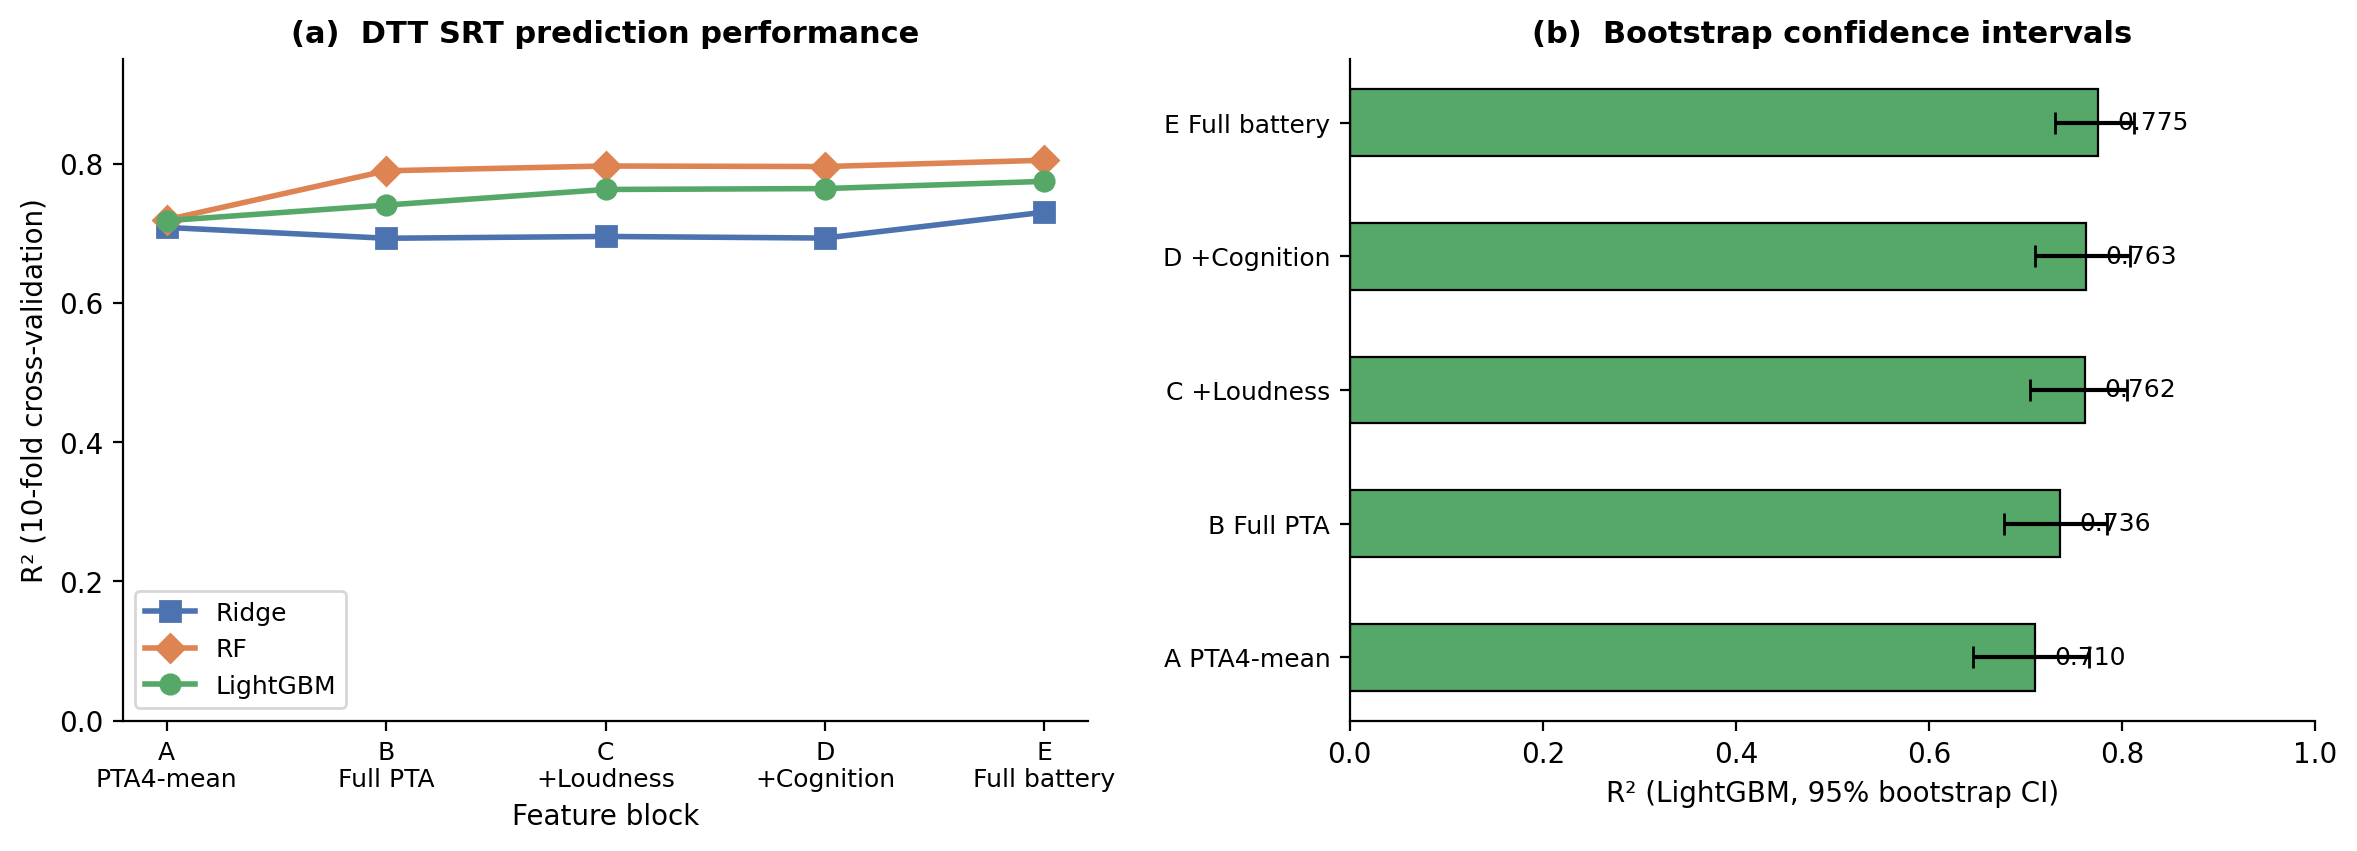
\includegraphics[width=\textwidth]{fig2_benchmark.png}
  \caption{\textbf{DTT SRT prediction performance across feature blocks and
  models.}  \textbf{(a)}~Ten-fold CV $R^2$ for all model\,$\times$\,block
  combinations.  Ensemble methods benefit from extended blocks; Ridge
  performance is more stable.  \textbf{(b)}~Bootstrap 95\% confidence
  intervals for LightGBM $R^2$ by block; intervals partially overlap
  between Blocks~B and C, indicating a consistent but moderate benefit from
  loudness features.}
  \label{fig:benchmark}
\end{figure*}

\begin{figure*}[htbp]
  \centering
  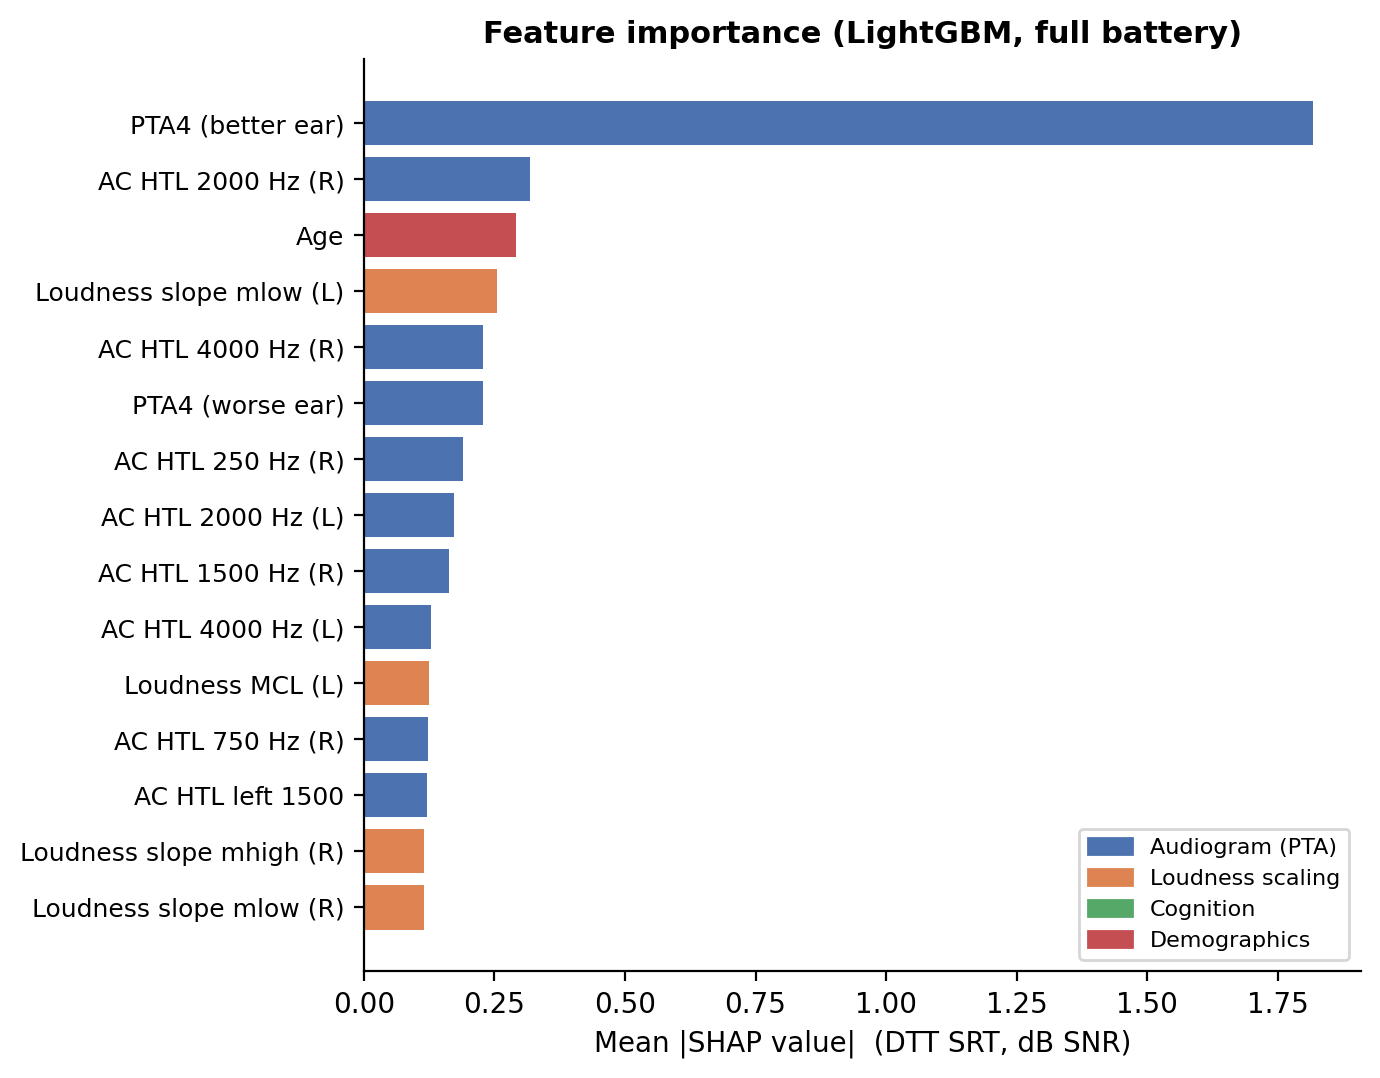
\includegraphics[width=0.75\textwidth]{fig3_shap.png}
  \caption{\textbf{SHAP feature importance (LightGBM, Block~E, top~15
  features).}  Colours indicate feature type: blue\,=\,audiogram, orange\,=\,loudness
  scaling, green\,=\,cognition, red\,=\,demographics.  Beyond the dominant
  PTA4 summary, age (rank~3) and loudness growth slope $m_\text{low}$
  (rank~4) are the most informative predictors.}
  \label{fig:shap}
\end{figure*}

\begin{figure*}[htbp]
  \centering
  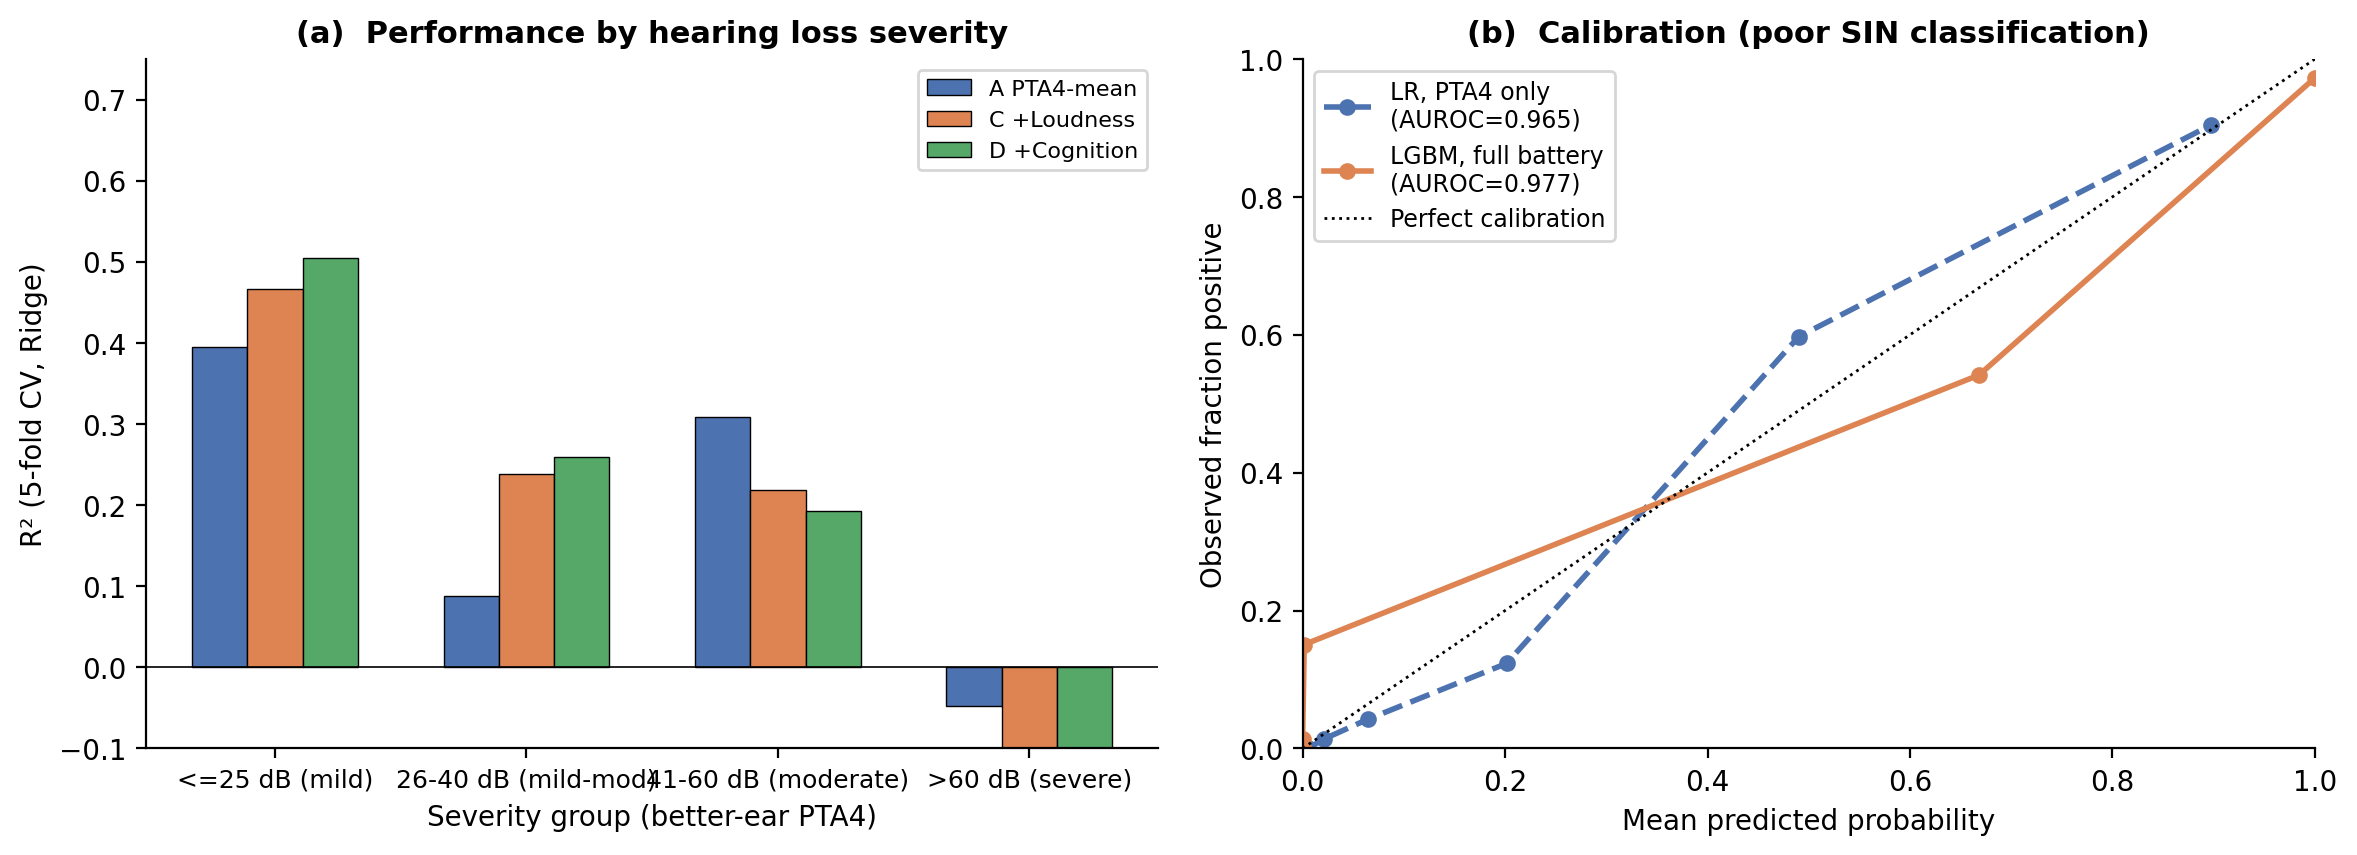
\includegraphics[width=\textwidth]{fig4_subgroup_calibration.png}
  \caption{\textbf{Severity-stratified analysis and calibration.}
  \textbf{(a)}~Within-stratum 5-fold Ridge $R^2$ for Block~A (PTA4 only)
  and Block~E (full battery).  The benefit of extended assessment is
  concentrated in mild hearing loss (26--40\,dB), where PTA4 alone explains
  only 9\% of SIN variance.
  \textbf{(b)}~Calibration curves for LR (Block~A) and LightGBM (Block~E)
  predicting poor SIN performers; both models show close agreement with the
  diagonal.}
  \label{fig:subgroup}
\end{figure*}

\begin{figure*}[htbp]
  \centering
  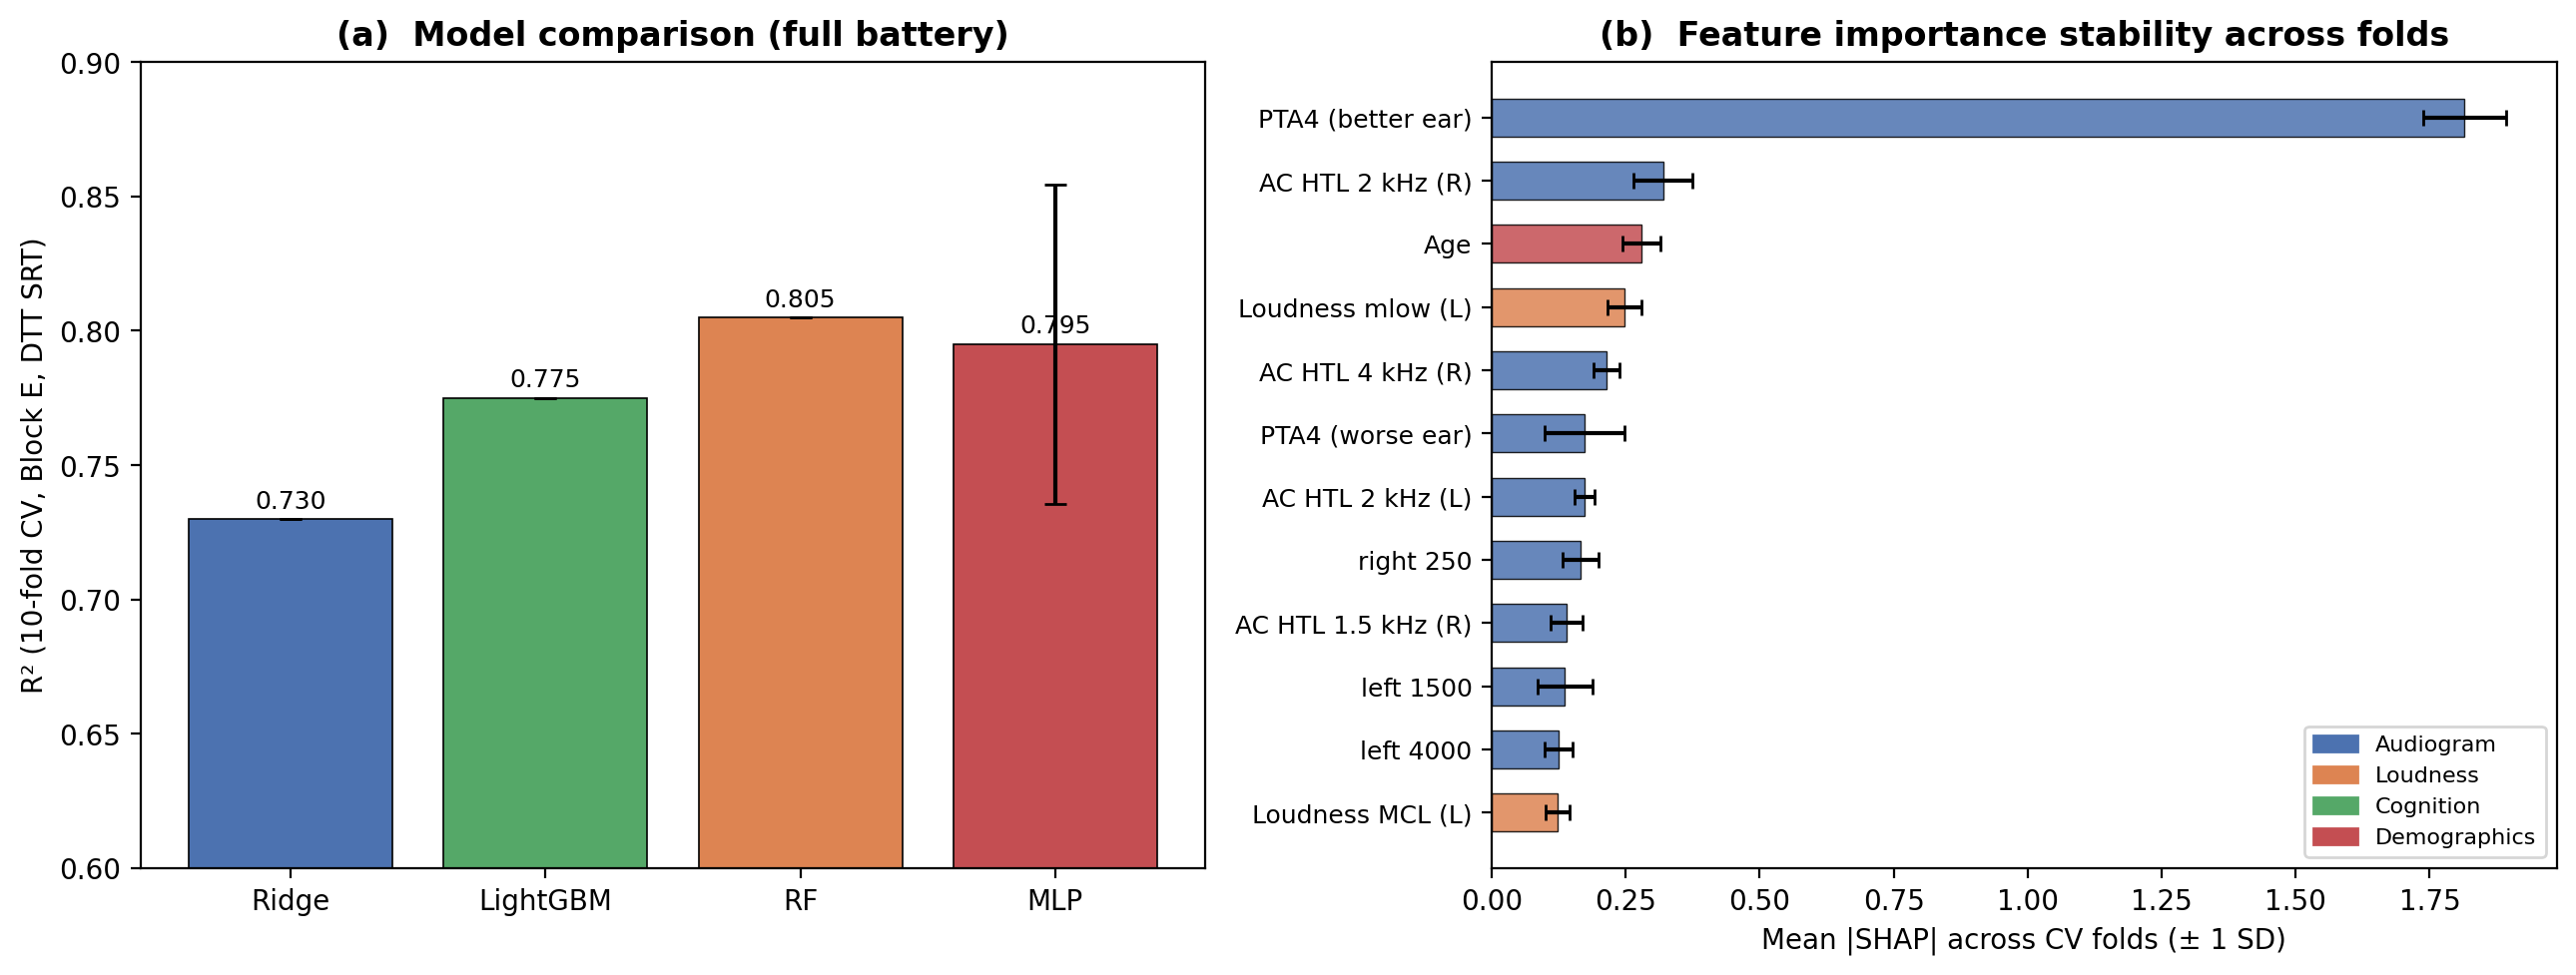
\includegraphics[width=\textwidth]{fig6_model_comparison_stability.png}
  \caption{\textbf{Model comparison and SHAP stability.}
  \textbf{(a)}~Block~E $R^2$ for Ridge, LightGBM, RF, and MLP; error bar
  for MLP shows $\pm$1~SD across folds.
  \textbf{(b)}~Mean absolute SHAP values with fold-level SD ($\pm$1~SD
  error bars); top features have coefficient-of-variation\,$<$\,0.15,
  confirming ranking stability.}
  \label{fig:comparison}
\end{figure*}

\begin{figure*}[htbp]
  \centering
  
\includegraphics[width=\textwidth]{fig5_crosscohort.png}
  \caption{\textbf{Cross-cohort validation: OHHR $\to$ NHANES.}
  \textbf{(a)}~AUROC for predicting NHANES self-reported hearing difficulty
  (AUQ054) by feature set.  Adding age to PTA4 raises AUROC from 0.758 to
  0.815.
  \textbf{(b)}~Distribution of predicted P(poor SIN) by NHANES AUQ054
  category (1\,=\,excellent, 5\,=\,a lot of trouble, 6\,=\,deaf); predicted
  risk increases monotonically with hearing difficulty category.
  \textbf{(c)}~OOF calibration curves on OHHR for PTA4-only and PTA4+Age
  classifiers.}
  \label{fig:crosscohort}
\end{figure*}

%% SUPPLEMENTARY
\clearpage
\section*{Supplementary Information}

\setcounter{table}{0}
\renewcommand{\thetable}{S\arabic{table}}

\begin{table}[htbp]
\caption{\textbf{Supplementary Table~S1.} Participant characteristics
($N=581$).}
\label{tab:demo_supp}
\centering\small
\begin{tabular}{lc}
\toprule
Characteristic & Value (mean\,$\pm$\,SD or $n$ (\%)) \\
\midrule
Age (years)                    & $67.5 \pm 12.0$ \\
Sex (male)                     & 326 (56.1\%) \\
Better-ear PTA4 (dB HL)        & $31.3 \pm 17.2$ \\
DTT SRT (dB SNR)               & $-4.60 \pm 4.16$ \\
GST SRT (dB SNR)               & $-1.46 \pm 3.11$ \\
DemTect score (0--18)          & $15.8 \pm 2.3$ \\
Verbal intelligence (WortSchatz) & $31.5 \pm 4.9$ \\
Poor SIN (DTT SRT $>-2$\,dB)  & 122 (21.0\%) \\
\midrule
\multicolumn{2}{l}{\textit{Severity (better-ear PTA4):}} \\
$\leq$25\,dB (normal/near-normal) & 228 (39.2\%) \\
26--40\,dB (mild)              & 174 (29.9\%) \\
41--60\,dB (moderate)          & 148 (25.5\%) \\
$>$60\,dB (severe/profound)    & 31 (5.3\%) \\
\bottomrule
\end{tabular}
\end{table}

\end{document}
